\documentclass[xcolor=table,dvipsnames]{beamer}

\usepackage{lscape, amsmath, amsfonts, amssymb, setspace, theorem, wrapfig, graphicx, float, multirow, subfig, color, rotating, multicol, datetime, natbib, venndiagram, pstricks, xkeyval, tikz, etoolbox, verbatim, pgf, tikz, pgfplots, mathrsfs, nth}

\usepackage{listings}
\usepackage{xcolor}
\usetikzlibrary{arrows}

\definecolor{codegreen}{rgb}{0,0.6,0}
\definecolor{codegreengray}{rgb}{0,0.4,0}
\definecolor{codegray}{rgb}{0.5,0.5,0.5}
\definecolor{codeblue}{rgb}{0.00,0,0.82}
\definecolor{backcolour}{rgb}{0.95,0.95,0.92}
\definecolor{jeopardy}{rgb}{.24,.47,.914}

\lstdefinestyle{mystyle}{
    backgroundcolor=\color{backcolour},   
    commentstyle=\color{codegreengray},
    numberstyle=\tiny\color{codegray},
    stringstyle=\color{codegreen},
    basicstyle=\ttfamily\footnotesize,
    breakatwhitespace=false,         
    breaklines=true,                 
    captionpos=b,                    
    keepspaces=true,                 
    numbers=left,                    
    numbersep=5pt,                  
    showspaces=false,                
    showstringspaces=false,
    showtabs=false,                  
    tabsize=2
}
 
\lstset{style=mystyle}

\title{GV300 - Quantitative Political Analysis}
\subtitle{University of Essex - Department of Government}
\date{Week 23 -- 2 March, 2020}				% or you can specify a date, just write it down instead of "\today"
\author{Lorenzo Crippa} 

\usetheme[progressbar=frametitle]{metropolis}
\usecolortheme{seahorse}						% try others: wolverine; crane...


\begin{document}

\begin{frame}[plain]
\begin{center}
\titlepage
\end{center}
\end{frame}

\begin{frame}{NSS survey}
\begin{center}

\includegraphics[scale=0.36]{pictures/week_23_NSS.pdf}
\end{center}
\end{frame}

\begin{frame}{Today's activity}
\begin{itemize}
\item Today we work on panel data. We use the dataset \texttt{panelModelsData\_{}rFile.dta} that you find on Moodle. \pause
\item Download the dataset and open it into R or Stata \pause
\item Data on 595 U.S. workers, measured at different points in time \pause
\item Consider only the first 100 workers, get rid of the rest of the data
\end{itemize}
\end{frame}

\begin{frame}
\frametitle{Analysis}
\begin{enumerate}
\item Causal identification \pause
	\begin{itemize}
	\item[(a)] We want to explain $log(wage)$ (\texttt{lwage}) as a function of at least experience (\texttt{exp}) and education (\texttt{ed}) \pause
	\item[(b)] What problem of identification do panel data help solving? \pause
	\end{itemize}
\item Data description \pause
	\begin{itemize}
	\item[(a)] Summary statistics and plots as usual \pause
	\item[(b)] Today we have lots of information: we also want to summarize variation of data between units, within units and overall \pause
	\end{itemize}
\item Data analysis \pause
	\begin{itemize}
	\item[(a)] Run a pooled, a fixed-effect and a random-effect model \pause
	\item[(b)] Remember to use robust standard errors. Are robust standard errors enough or should we do something more? \pause
	\item[(c)] Compare the results and discuss which model best fits data based on point 2(b).
	\end{itemize}
\end{enumerate}
\end{frame}

\section{1. Causal identification}

\begin{frame}{1(a) and (b) -- Causal model}
\begin{center}
\begin{tikzpicture}[line cap=round,line join=round,>=triangle 45,x=1cm,y=1cm]
\clip(2,-1) rectangle (7.7,2.5);
\draw [->,line width=0.6pt] (3,0) -- (6.9,0);
\draw [->,line width=0.6pt] (5,2) -- (3.1,0.1);
\draw [->,line width=0.6pt] (5,2) -- (6.9,0.1);
\begin{scriptsize}
\draw [fill=black] (3,0) circle (1.5pt);
\draw[color=black] (2.8,0.33) node {$Edu$};
\draw [fill=black] (7,0) circle (1.5pt);
\draw[color=black] (7.3,0.33) node {$Wage$};
\draw [fill=black] (5,2) circle (1.5pt);
\draw[color=black] (5,2.31) node {$X$};
\end{scriptsize}
\end{tikzpicture}  \pause
\end{center}
\begin{itemize}
\item Suppose $X$ is a set of confounders that make each specific unit \textit{idiosyncratic} both in treatment and outcome variables \pause
\item Then panel data help us identify the causal effect of $Edu$ on $Wage$ because they allow us to include a fixed (random) effect and control for it. \pause
\item \textbf{BUT} fixed/random effects are no solution for all other types of confounders (non-idiosyncratic)!
\end{itemize}
\end{frame}

\section{2. Data description}

\begin{frame}{2(a) -- Summary statistics}
\begin{table}[!htbp] \centering 
\resizebox{110mm}{35mm}{
\begin{tabular}{@{\extracolsep{5pt}}lccccccc} 
\\[-1.8ex]\hline 
\hline \\[-1.8ex] 
Variable & \multicolumn{1}{c}{N} & \multicolumn{1}{c}{Mean} & \multicolumn{1}{c}{St. Dev.} & \multicolumn{1}{c}{Min} & \multicolumn{1}{c}{Pctl(25)} & \multicolumn{1}{c}{Pctl(75)} & \multicolumn{1}{c}{Max} \\ 
\hline \\[-1.8ex] 
\texttt{id} & 700 & 50.500 & 28.887 & 1 & 25.8 & 75.2 & 100 \\ 
\texttt{t} & 700 & 4.000 & 2.001 & 1 & 2 & 6 & 7 \\ 
\texttt{occ} & 700 & 0.486 & 0.500 & 0 & 0 & 1 & 1 \\ 
\texttt{lwage} & 700 & 6.704 & 0.492 & 5.165 & 6.397 & 7.003 & 8.049 \\ 
\texttt{ed} & 700 & 13.040 & 2.995 & 4 & 12 & 16 & 17 \\ 
\texttt{exp} & 700 & 21.280 & 10.788 & 1 & 12 & 30 & 51 \\ 
\texttt{exp2} & 700 & 569.060 & 508.066 & 1 & 144 & 900 & 2,601 \\ 
\texttt{south} & 700 & 0.327 & 0.470 & 0 & 0 & 1 & 1 \\ 
\texttt{smsa} & 700 & 0.627 & 0.484 & 0 & 0 & 1 & 1 \\ 
\texttt{fem} & 700 & 0.130 & 0.337 & 0 & 0 & 0 & 1 \\ 
\texttt{union} & 700 & 0.321 & 0.467 & 0 & 0 & 1 & 1 \\ 
\hline \\[-1.8ex] 
\end{tabular} 
}
\end{table} 
\end{frame}

\begin{frame}{2(a) -- Usual ways of describing data}
We can use plots as usual to describe our data. For instance: \pause
\begin{center}
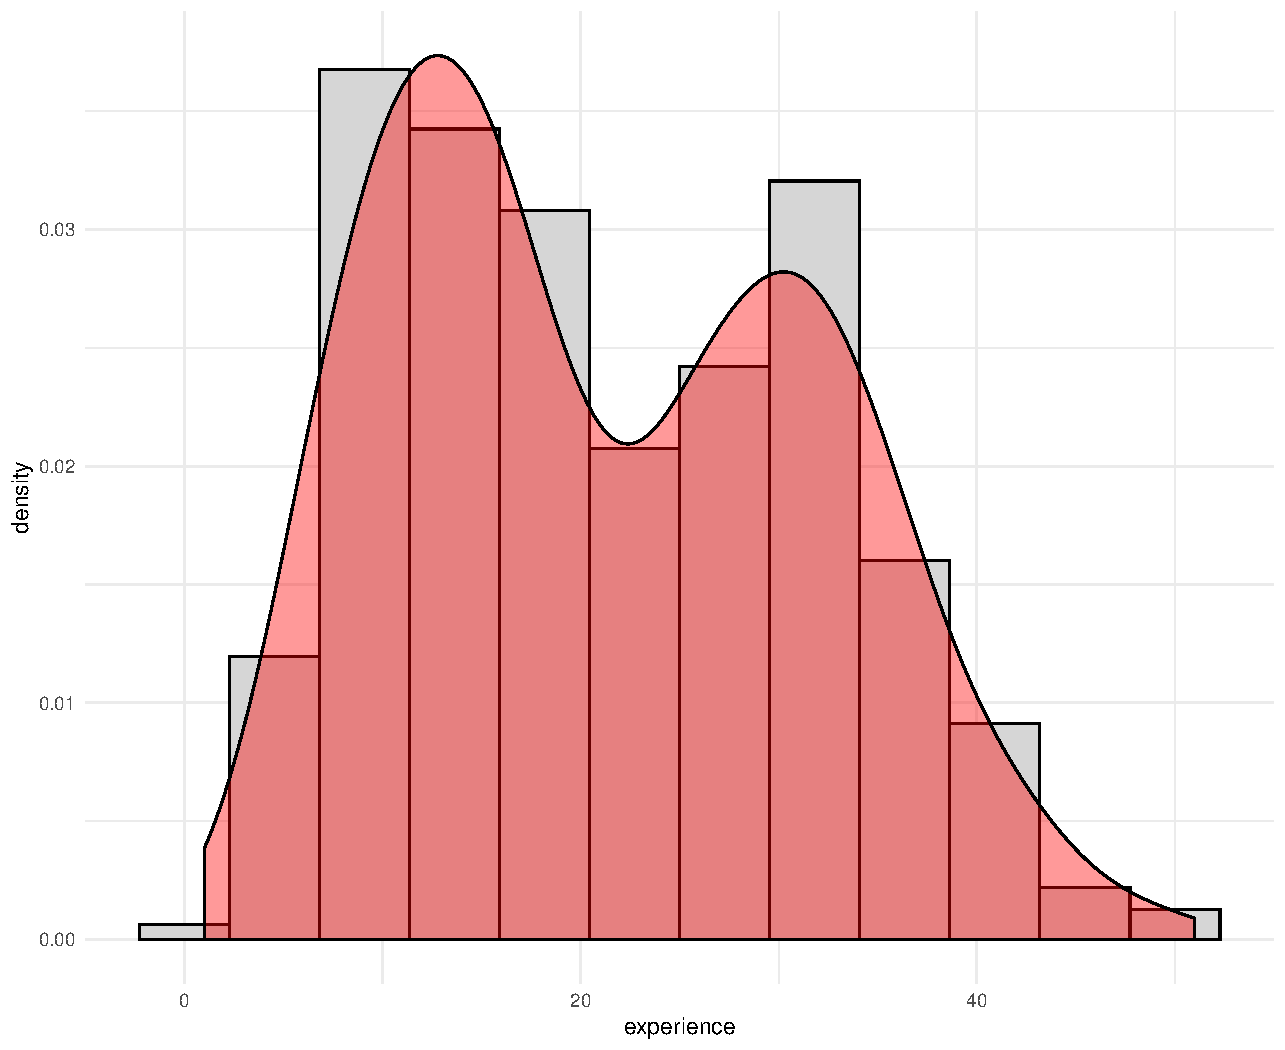
\includegraphics[scale=0.4]{pictures/week_23_histdens.pdf}
\end{center}
\end{frame}

\begin{frame}{With \texttt{ggplot2} you can do basically everything}
With \texttt{ggplot2} the limit is your imagination (sorry Stata users): \pause
\begin{center}
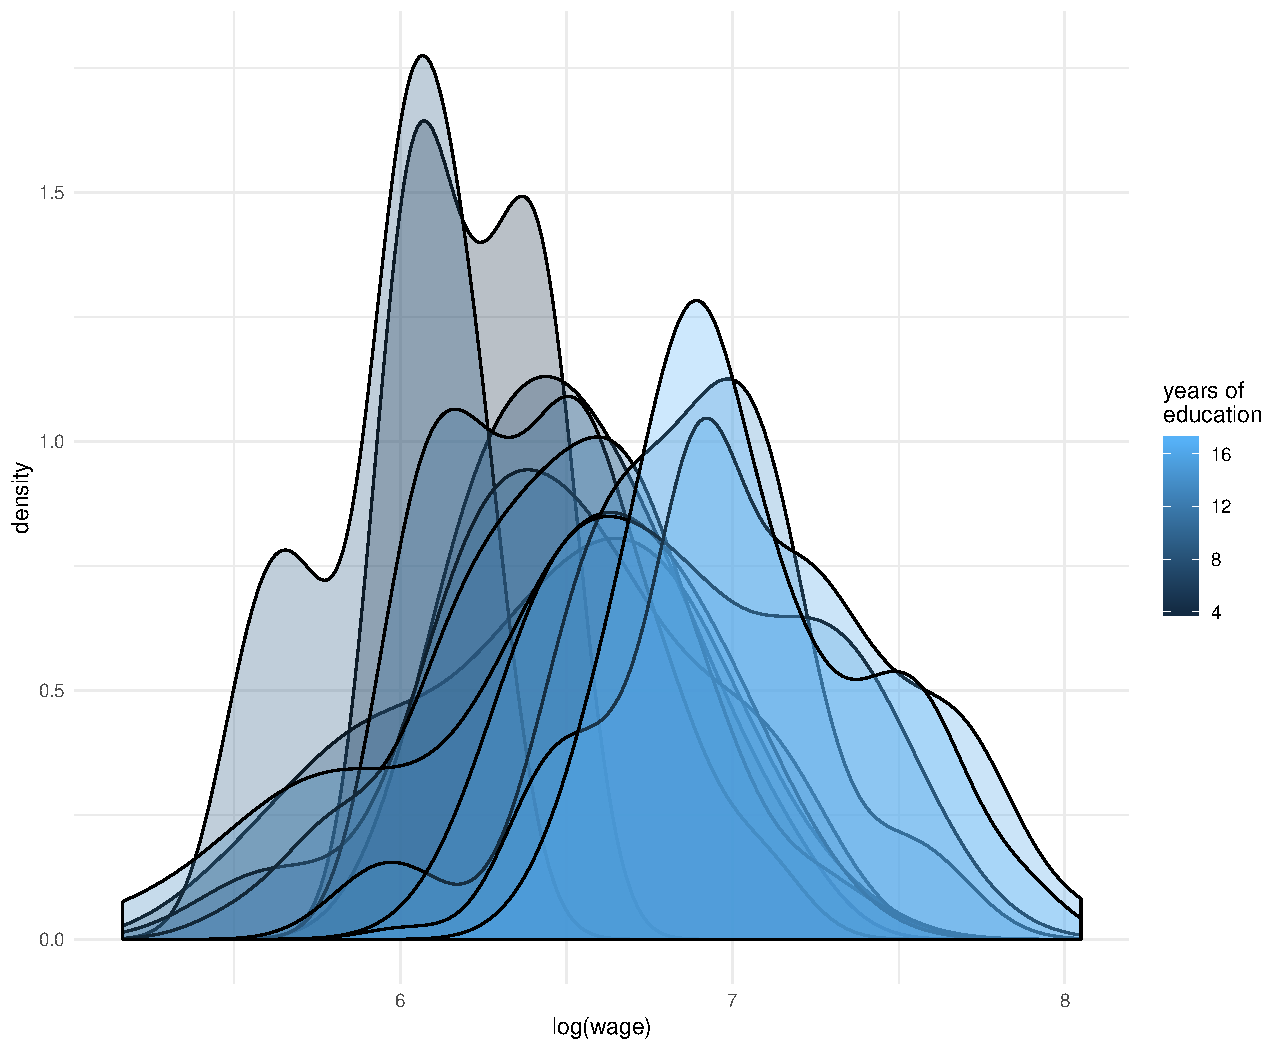
\includegraphics[scale=0.4]{pictures/week_23_dens.pdf}
\end{center}
\end{frame}

\begin{frame}{2(a) -- Scatterplots}
What does the following scatterplot tell you?
\begin{center}
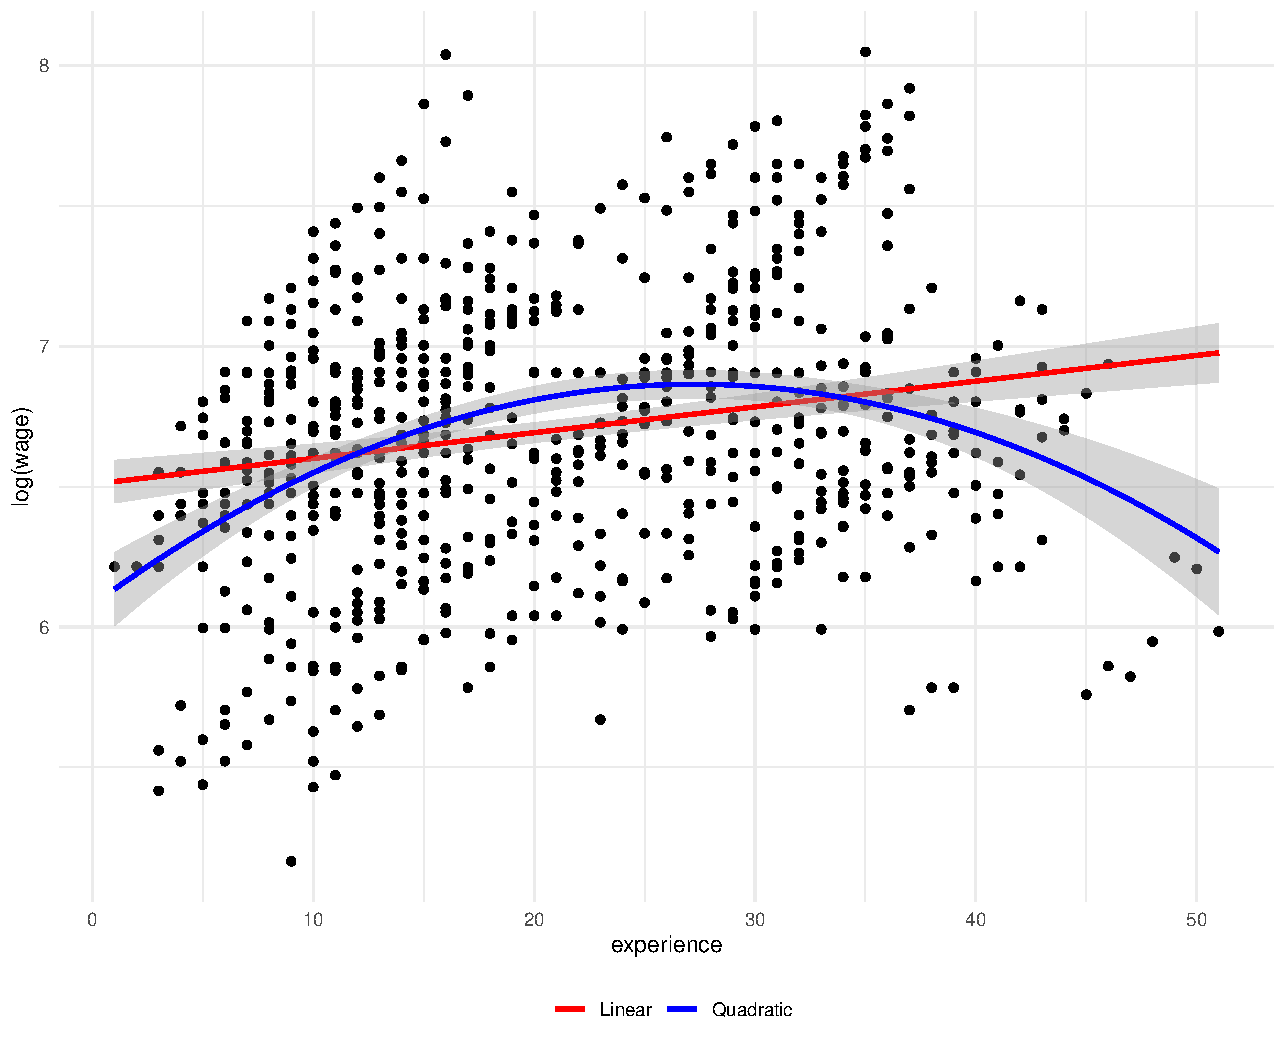
\includegraphics[scale=0.33]{pictures/week_23_badscatter.pdf}
\end{center} \pause
Our usual linear model doesn't really seem to fit this cloud. Why?
\end{frame}

\begin{frame}{2(b) -- Fixed effect}
Take a look at this graph (only first 20 individuals). What does it suggest about the relationship we are studying?
\begin{center}
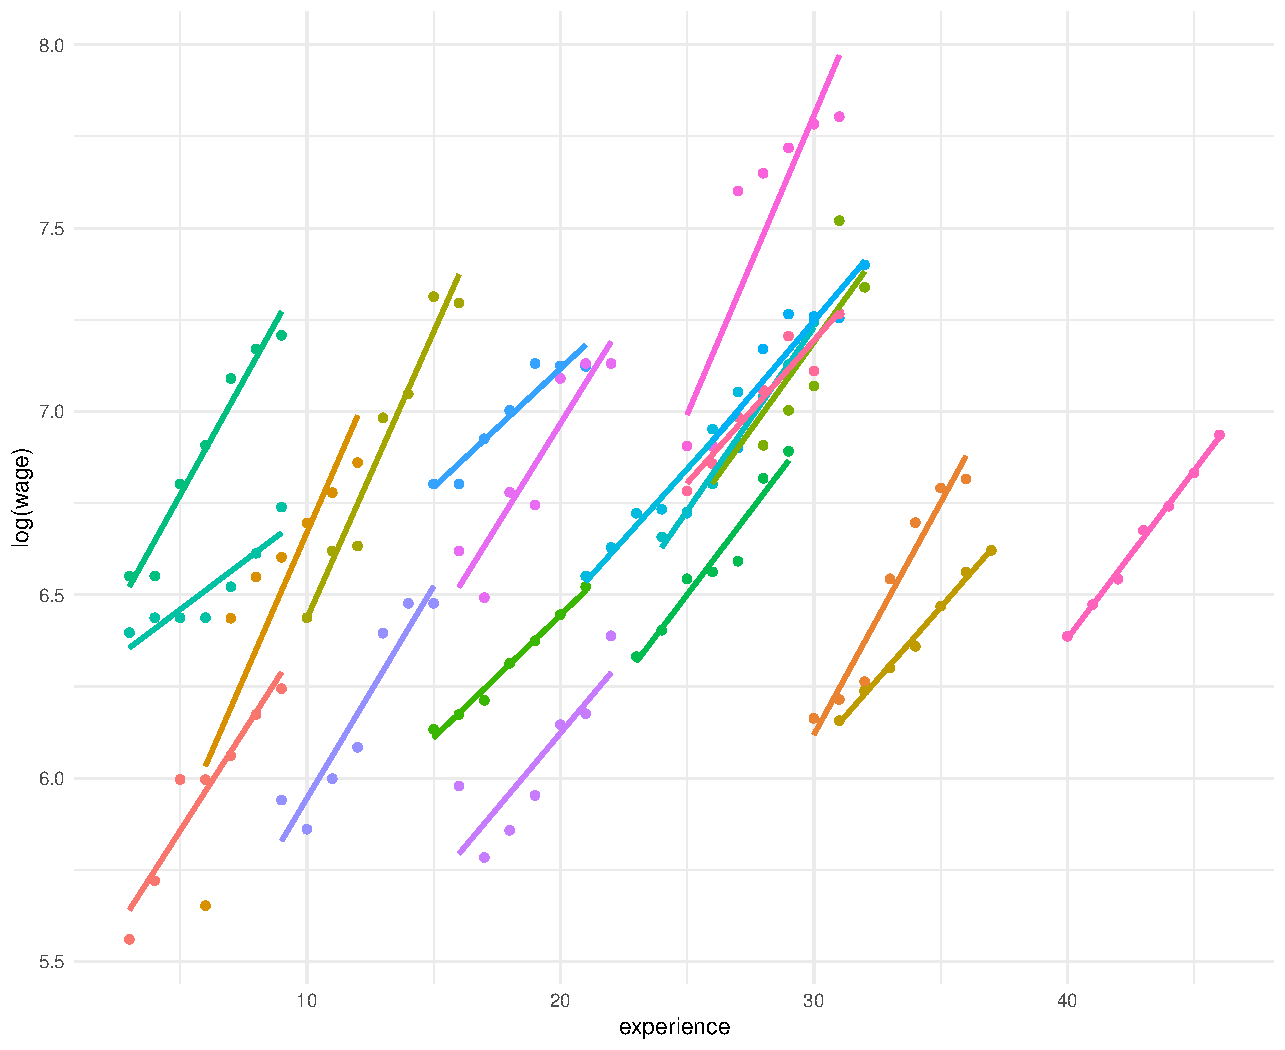
\includegraphics[scale=0.28]{pictures/week_23_groupline.pdf}
\end{center} \pause
The slopes of the regression lines by individual seem similar, only between-units intercepts are different!
\end{frame}

\begin{frame}{2(b) -- Fixed effect}
Now look at the following (all 100 individuals, plus pooled):
\begin{center}
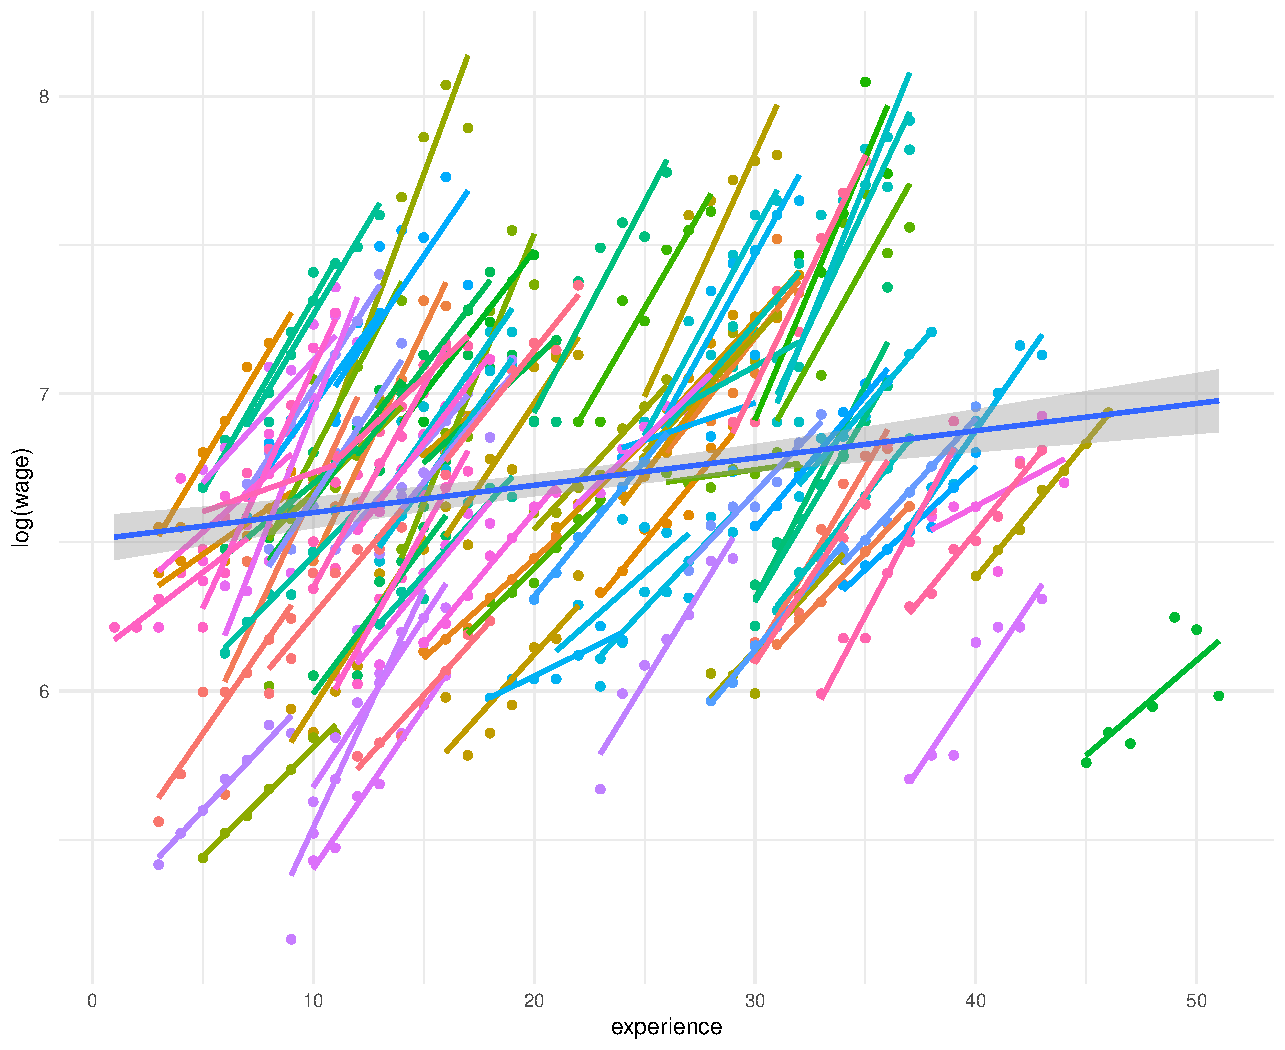
\includegraphics[scale=0.31]{pictures/week_23_fixed_effect.pdf}
\end{center} \pause
A typical example of a fixed effect: slopes and intercepts of lines by individuals are different from those of pooled line.
\end{frame}

\begin{frame}{Fixed and random effect made intuitive}
\begin{itemize}
\item You can have both unit- and time-fixed (random) effect \pause
\item Use fixed effect when intercepts \textbf{and} slopes of reg lines by units (or time) $\neq$ intercept and slope of the pooled reg line \pause
\item Use random effect when \textbf{only} intercepts of reg lines by units (or time) $\neq$ intercept of the pooled reg line. Slopes $\approx$ to the slope of the pooled reg (with some variation) \pause 
\item \textbf{Both} fixed and random have different intercepts of the reg lines by units (or time)! \pause
\item Intuitively: you include a fixed effect in a pooled model $\rightarrow$ you have no clue of what's the difference between units, so you get rid of it. \pause Random effect $\rightarrow$ you can explain part of it.
\end{itemize}
\end{frame}


\begin{frame}{2(b) -- What about time?}
Are the time-points we have absolutely different from each others?
\begin{center}
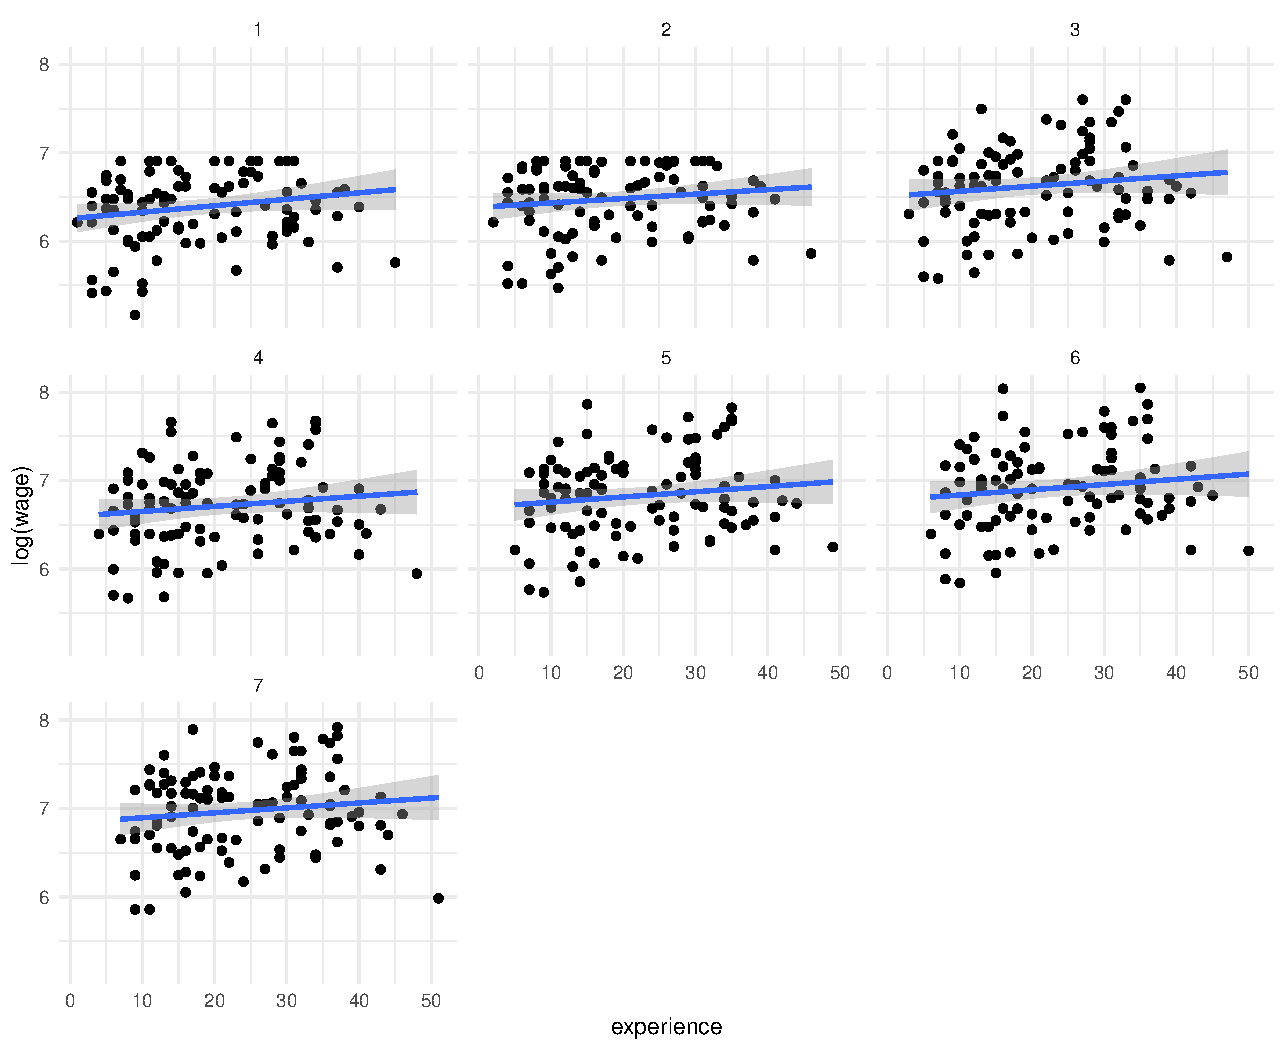
\includegraphics[scale=0.33]{pictures/week_23_timescatter.pdf}
\end{center} \pause
In R we can even animate our graphs using \texttt{gganimate}!
\end{frame}

\begin{frame}{2(b) -- Time fixed effect?}
Look at the following lines: is a time-fixed effect appropriate here?
\begin{center}
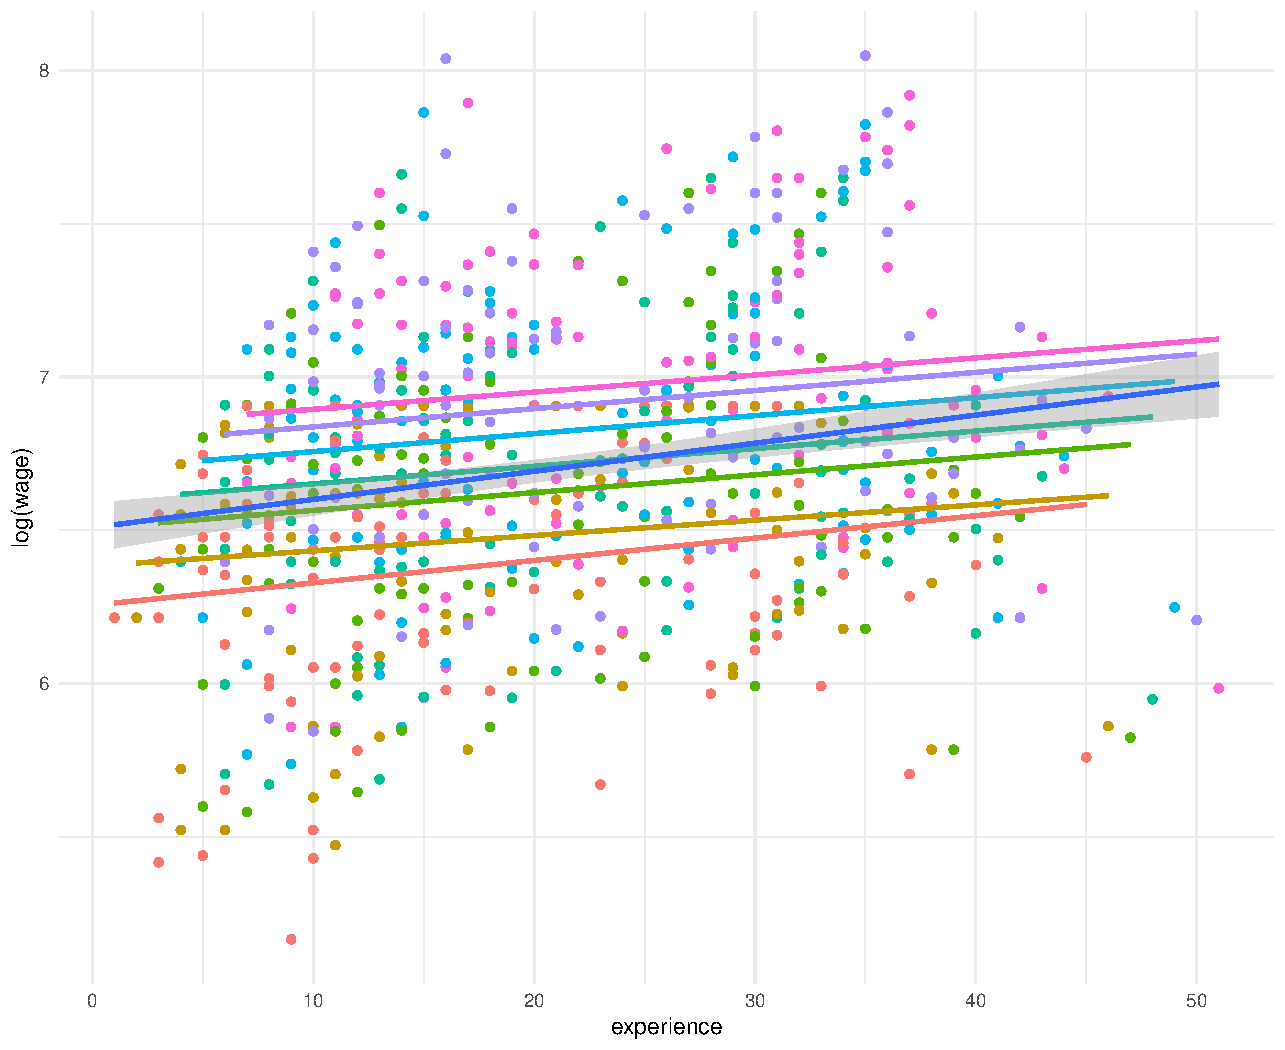
\includegraphics[scale=0.4]{pictures/week_23_yearfe.pdf}
\end{center}
\end{frame}


\begin{frame}[fragile]
\frametitle{2(b) -- Within, between and overall variation}
We can get statistics about within, between and overall variation of a selected number of variables (see R script): \pause

\begin{small}
\begin{verbatim}
within.variation
   t     lwage   ed     exp     exp2    wks
   2.00	 0.235   0      2.00    95.2    3.85
   
between.variation
   t     lwage   ed     exp     exp2    wks
   0     0.434   3.01   10.6    501.    3.24
  
overall.variation
   t     lwage   ed     exp     exp2    wks
   2.00  0.492   3.00   10.8    508.    5.02
\end{verbatim}
\end{small}
\end{frame}

\section{3. Data analysis}

\begin{frame}{Fixed effect: dummies}
You introduce a fixed effect to perform a within-unit (or time) estimation. \pause Suppose you have $k$ different units. Mathematically:
$$Y_{it} = a_0 + \mathbf{X'_{it} b} + a_1 D_1 + a_2 D_2 + \ldots + a_{k-1} D_{k-1} + e_{it} $$
$$\mathbf{D} = D_1, D_2, \ldots, D_k =
\left[
\begin{array}{cccc}
1			& 0			& \ldots	& 0 		\\
1 			& 0	 		& \ldots	& 0 		\\
0			& 1			& \ldots	& 0 		\\
0			& 1			& \ldots	& 0 		\\
\vdots 		& \vdots	& \ddots 	& \vdots	\\
0			& 0			& \ldots	& 1			\\
0 			& 0			& \ldots	& 1 		\\
\end{array}
\right]
$$ \pause
The matrix has size $N \times k$. Your software will exclude one dummy (thus $k-1$) or the intercept $a_0$ to avoid multicollinearity
\end{frame}

\begin{frame}{Fixed effect: entity demeaned}
Problems in estimating a fixed effect using dummies: \pause
\begin{enumerate}
\item You easily run out of degrees of freedom \pause
\item Computationally heavy
\end{enumerate} \pause

Solution: entity-demeaned FE (what your softwares do)

\begin{center}
$Y_{it} = a_0 + \mathbf{X'_{it} b} + u_{it}$ \pause $\rightarrow$ $Y_{it} = a_0 + \mathbf{X'_{it} b} + a_i + e_{it}$ 
\end{center} \pause
$$\overline{Y}_{i} = a_0 + \mathbf{\overline{X}'_{i} b} + a_i + \overline{e}_{i} $$ \pause
We can now do the group demeaning:
$$(Y_{it} - \overline{Y}_{i}) = (\mathbf{X'_{it}}-\mathbf{\overline{X}'_i}) \mathbf{b} + (a_i - a_i) + (e_{it} - \overline{e}_{i})$$ \pause
Thus we get rid of between-unit variation ($a_i - a_i=0$)
\end{frame}

\begin{frame}{Maths on random effect}
Random effect:
$$(Y_{it}-\hat{\theta}_i\overline{Y}_i) = (1-\hat{\theta}_i)a_0 + (\mathbf{X}_{it}-\hat{\theta}_i\overline{\mathbf{X}_{i}})'\mathbf{b}+[(1-\hat{\theta}_i)a_i+(e_{it}-\hat{\theta}_i\overline{e}_i)]$$ \pause

where $\hat{\theta}_i$ is an estimate of $$\theta_i = 1 - \sqrt{\frac{\sigma_e^2}{T_i\sigma^2_a+\sigma_e^2}}$$ \pause 

Assumption: $E(e_{it}|\mathbf{x}_{it})=0$ \pause

Notice that, for each covariate in $\mathbf{X_{it}}$, you have a (slightly) different slope for each unit $i$, depending on $\hat{\theta}_i$!
\end{frame}

\begin{frame}{From random effect to fixed effect and pooled model}
Now, consider:
$$(Y_{it}-\hat{\theta}_i\overline{Y}_i) = (1-\hat{\theta}_i)a_0 + (\mathbf{X}_{it}-\hat{\theta}_i\overline{\mathbf{X}_{i}})'\mathbf{b}+[(1-\hat{\theta}_i)a_i+(e_{it}-\hat{\theta}_i\overline{e}_i)]$$
$$\theta_i = 1 - \sqrt{\frac{\sigma_e^2}{T_i\sigma^2_a+\sigma_e^2}}$$ \pause

\begin{enumerate}
\item what if $\sigma^2_a\gg\sigma_e^2$ (huge between-unit variation)? \pause $\theta_i \rightarrow 1$: we are back to the entity-demeaned fixed effect! \pause
\item what if $\sigma^2_a\ll\sigma_e^2$ (minimal between-unit variation)? \pause $\theta_i \rightarrow 0$: we are back to the pooled model! \pause
\item in-between these extremes: random effect \pause
\end{enumerate}

Your software will usually provide to you an estimate of $\theta_i$ (or of the variance of slopes) and related tests. Check the output!
\end{frame}

\begin{frame}
\frametitle{3(c) -- Model comparison}
\begin{table}
\begin{center}
\resizebox{100mm}{40mm}{
\begin{tabular}{l c c c c }
\hline
 & Pooled & Pooled 			& Fixed  	& Random  \\
 &		  & (clustered SE)	& Effect	& Effect \\
\hline
(Intercept) & $4.72^{***}$  & $4.72^{***}$  &              & $3.20^{***}$ \\
            & $(0.15)$      & $(0.24)$      &              & $(0.33)$     \\
exp         & $0.06^{***}$  & $0.06^{***}$  & $0.11^{***}$ & $0.09^{***}$ \\
            & $(0.01)$      & $(0.01)$      & $(0.01)$     & $(0.01)$     \\
exp2        & $-0.00^{***}$ & $-0.00^{***}$ & $-0.00$      & $-0.00^{*}$  \\
            & $(0.00)$      & $(0.00)$      & $(0.00)$     & $(0.00)$     \\
wks         & $-0.00$       & $-0.00$       & $0.00^{*}$   & $0.00$       \\
            & $(0.00)$      & $(0.00)$      & $(0.00)$     & $(0.00)$     \\
ed          & $0.10^{***}$  & $0.10^{***}$  &              & $0.14^{***}$ \\
            & $(0.01)$      & $(0.01)$      &              & $(0.02)$     \\
\hline
Adj. R$^2$  & 0.43          & 0.43          & 0.70         & 0.52         \\
Num. obs.   & 700           & 700           & 700          & 700          \\
\hline
\multicolumn{5}{l}{\scriptsize{$^{***}p<0.01$, $^{**}p<0.05$, $^*p<0.1$}}
\end{tabular}
}
\end{center}
\end{table}
\end{frame}

\begin{frame}[fragile]
\frametitle{Fixed effect or random effect?}
We can perform a Hausman test to decide between FE and RE \pause
\begin{itemize}
\item $H_0$: difference between coefficients estimated in a fixed and random effect is not systematic \pause
\item Under $H_0$, RE will provide consistent \textbf{and efficient} estimates \pause
\item Under $H_1$, RE will provide inconsistent estimates \pause
\end{itemize}
In R (Stata is very similar, see script):
\begin{lstlisting}[language=R]
phtest(fe, re)

####################################################
# 	Hausman Test
#
# data:  lwage ~ exp + exp2 + wks + ed
# chisq = 3805.5, df = 3, p-value < 2.2e-16
# alternative hypothesis: one model is inconsistent
####################################################
\end{lstlisting}
\end{frame}

\begin{frame}{Final remarks}
Remember:
\begin{itemize}
\item Heteroskedasticity-robust standard errors are not enough anymore with panel data \pause
\item We should use \textbf{clustered} SEs (on our units) when we have panel data, otherwise we are not fixing serial correlation between units \pause
\item These SEs will \textbf{also} be robust to heteroskedasticity \pause
\item Look at the education variable. Why is it omitted from the fixed effect model? \pause 
\item Because for each respondent (within unit) education does not change! Thus there is no within-variation, and the within-variation is the only thing a fixed-effect looks at.
\end{itemize}
\end{frame}

\frame{
\frametitle{Conclusion}
\begin{center}
All clear? More questions? \\
Thanks and see you next week!
\end{center}
}

\end{document}